% ----------------------------------------------------------------------
\chapter{Erzeugnis}
% ----------------------------------------------------------------------
\section{Auslegung der grafischen Arbeitsoberfläche}

\begin{figure}[h!]
	\centering
	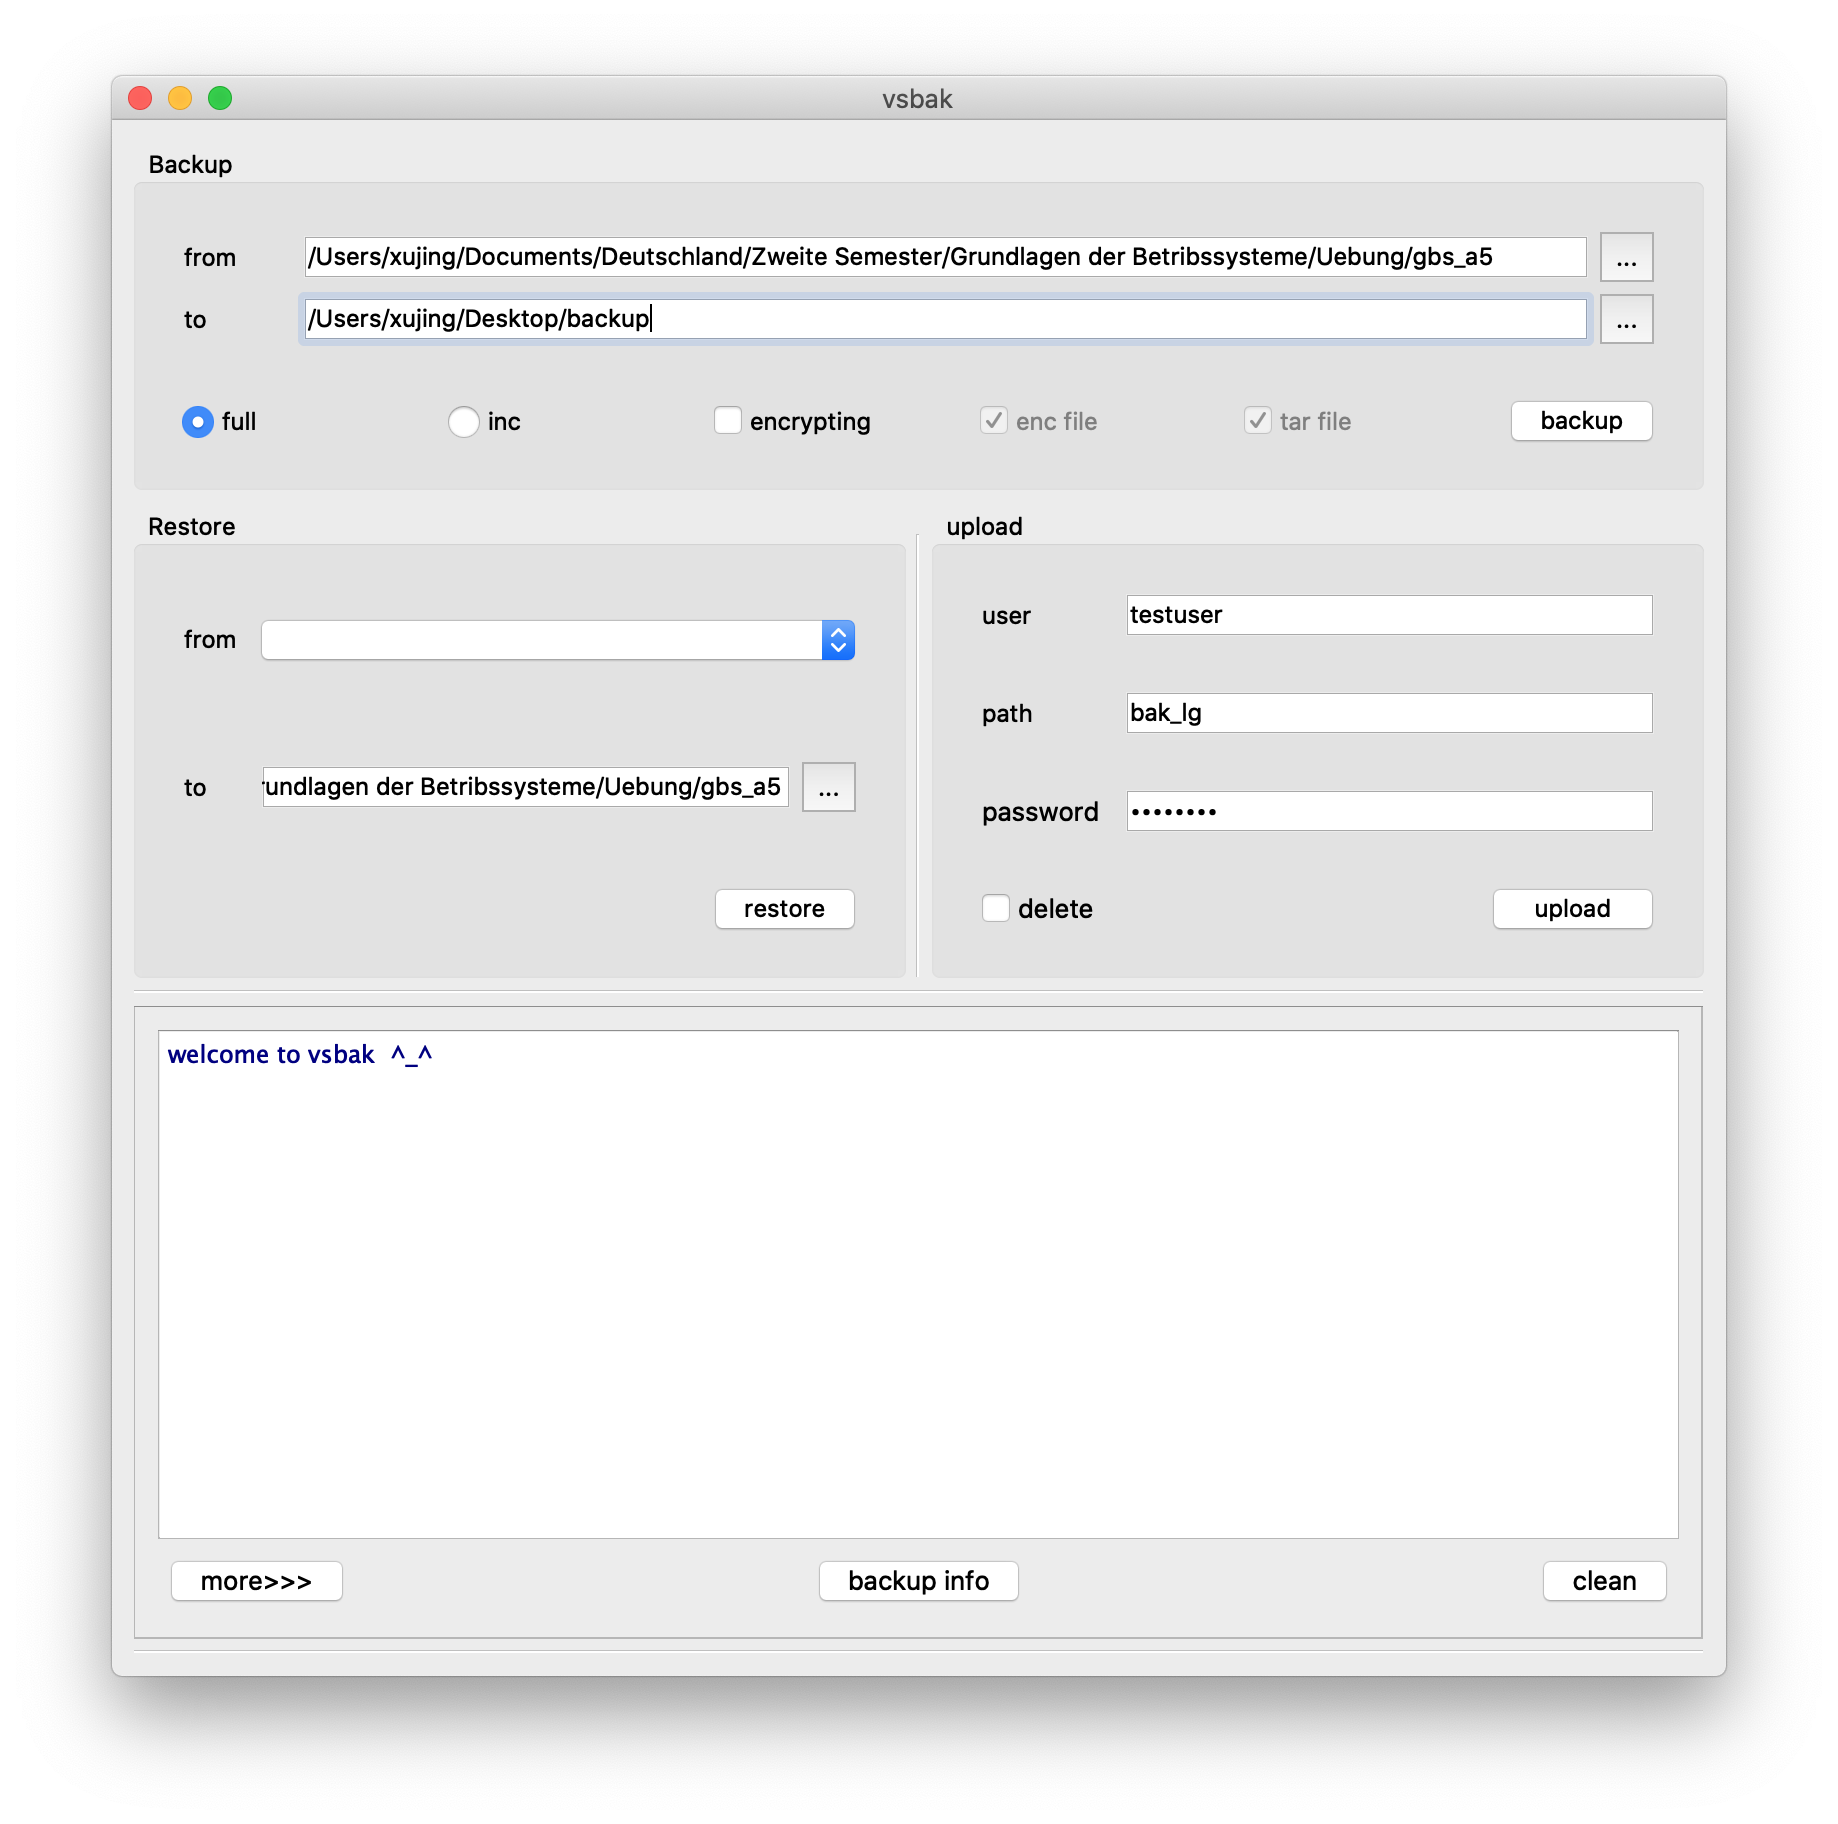
\includegraphics[width=0.8\textwidth]{bilder/vsbak_ui.png}
	\caption{die grafische Benutzeroberflaeche  }
	\label{Abbildung_3}
\end{figure}

Die Arbeitsoberfläche werden in 5 Arbeitsbereiche eingeteilt, auf die im Folgenden näher in den Einzelheiten eingegangen wird. (s. Abbildung \ref{Abbildung_3}). 

\begin{figure}[h!]
	\centering
	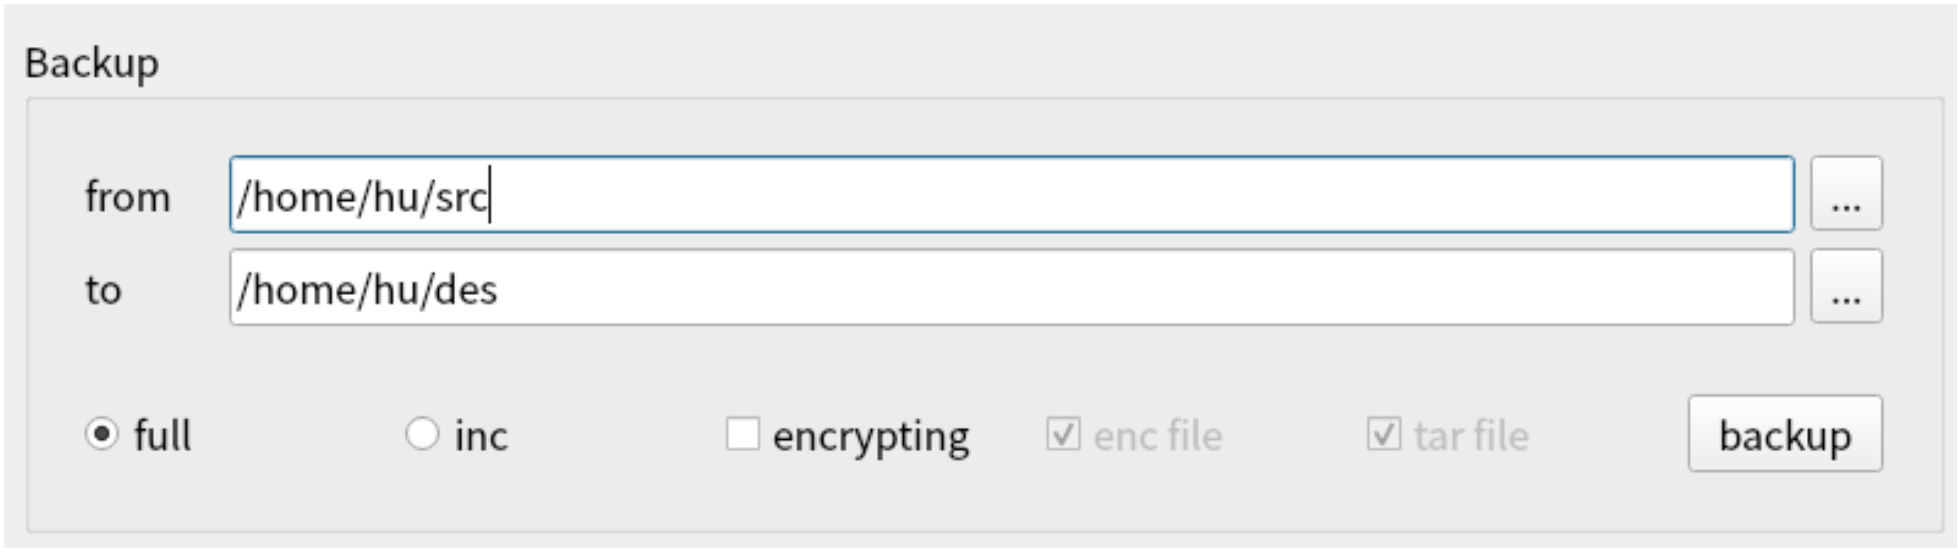
\includegraphics[width=0.8\textwidth]{bilder/backup.png}
	\caption{Der Bereich des Backups  }
	\label{Abbildung_4}
\end{figure}

Im Back-up Bereich lassen sich die Quellen- und Zieladresse bestimmen.  Mit den Kombinationen der im untenstehenden 2 Radio Buttons und 3 Checkboxes erfolgen  unterschiedliche Backup-Auswahl. Mit der “full” oder “inc”- Auswahl werden die Dateien komplett oder teilweise in die Zieladresse gesichert. Anschließend folgen die Verschlüsselung und Kompression. Mit dem „full“-Button wird eine ganze Datei im ausgewählten Ordner in die Zieladresse gesichert. Im Vergleich dazu ist die inkrementelle Sicherung durch die Auswahl  des “inc”-Buttons  zu erzielen. 
\par Die Verschlüsselung und Kompression lassen sich durch “encrypting” und “tar file” feststellen. Mit dem Häkchen im Checkbox des „enc file“- und „tar file“-Buttons werden die Nebendatei für Verschlüsselung und die komprimierte Datei deshalb in die Zieladresse gesichert.  Man kann die “enc file” und “tar file” aber erst willkürlich entfallen oder nicht, nachdem das „encrypting“- Button erstmals ausgewählt werden, weil die beiden nach der Initialisierung angekreuzt werden. (s. Abbildung \ref{Abbildung_4}).

\begin{figure}[h!]
	\centering
	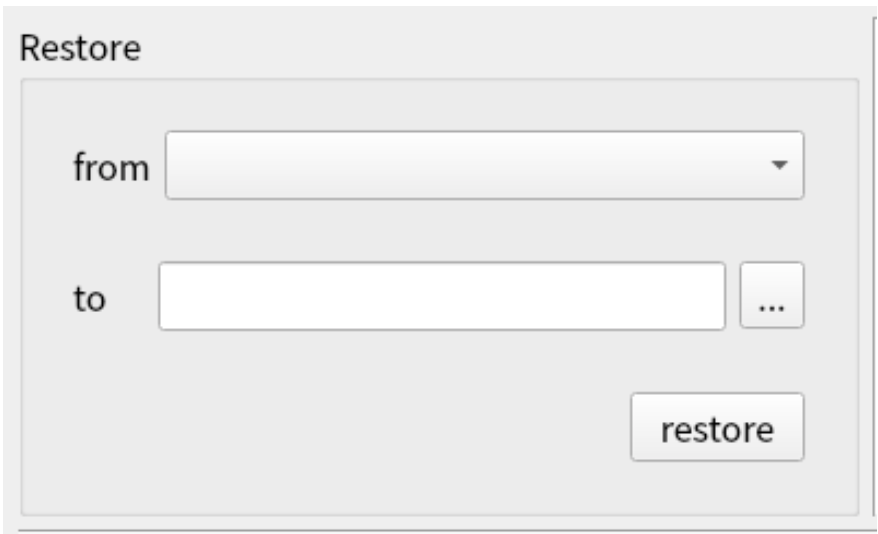
\includegraphics[width=0.4\textwidth]{bilder/restore.png}
	\caption{Der Bereich des Restores  }
	\label{Abbildung_5}
\end{figure}

Im Restore Bereich wird die bevorzugte Datei von der im Back-up bestimmten Zieladresse in eine neue Zieladresse wiederhergestellt. (s. Abbildung \ref{Abbildung_5}).

\begin{figure}[h!]
	\centering
	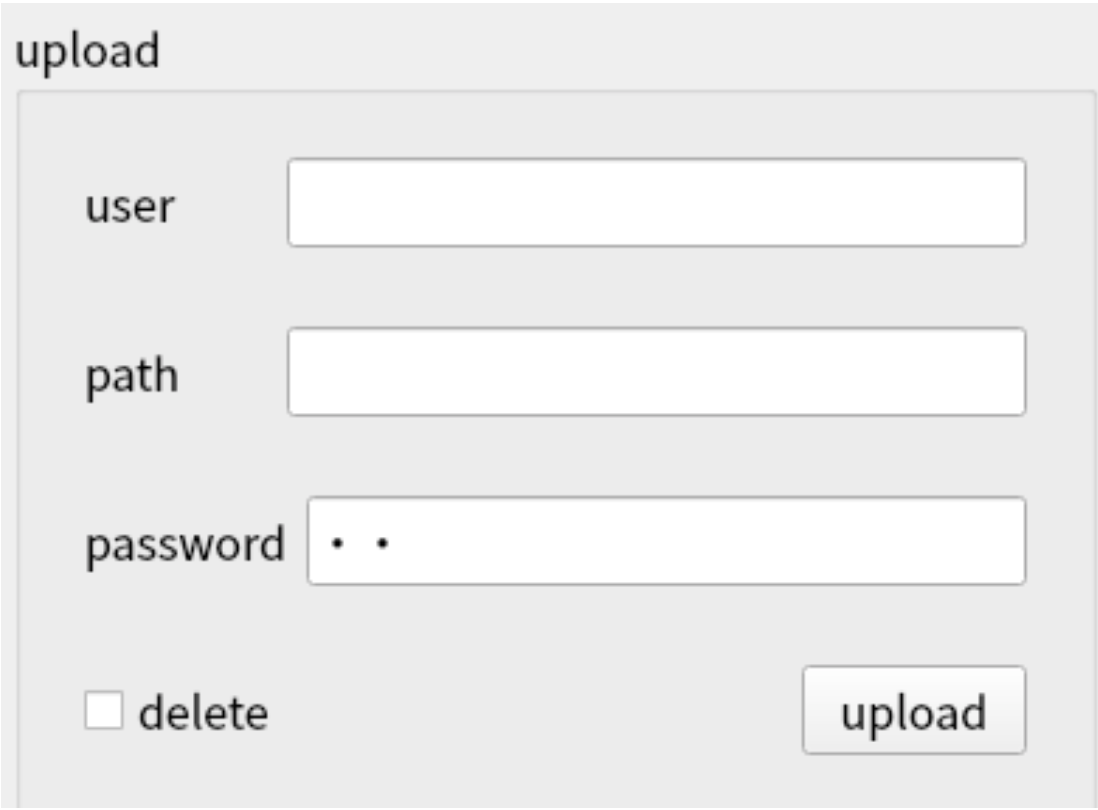
\includegraphics[width=0.4\textwidth]{bilder/upload.png}
	\caption{Der Bereich des Uploads  }
	\label{Abbildung_6}
\end{figure}

Ausschließlich 3 Eingabefelder für user, path und Passwort werden in Upload-Bereich integriert,  um die angeforderte Datei in das Internet hochzuladen. Das delete Button wird benutzt, um die uploadeten Dateien zu löschen. (s. Abbildung \ref{Abbildung_6})

\begin{figure}[h!]
	\centering
	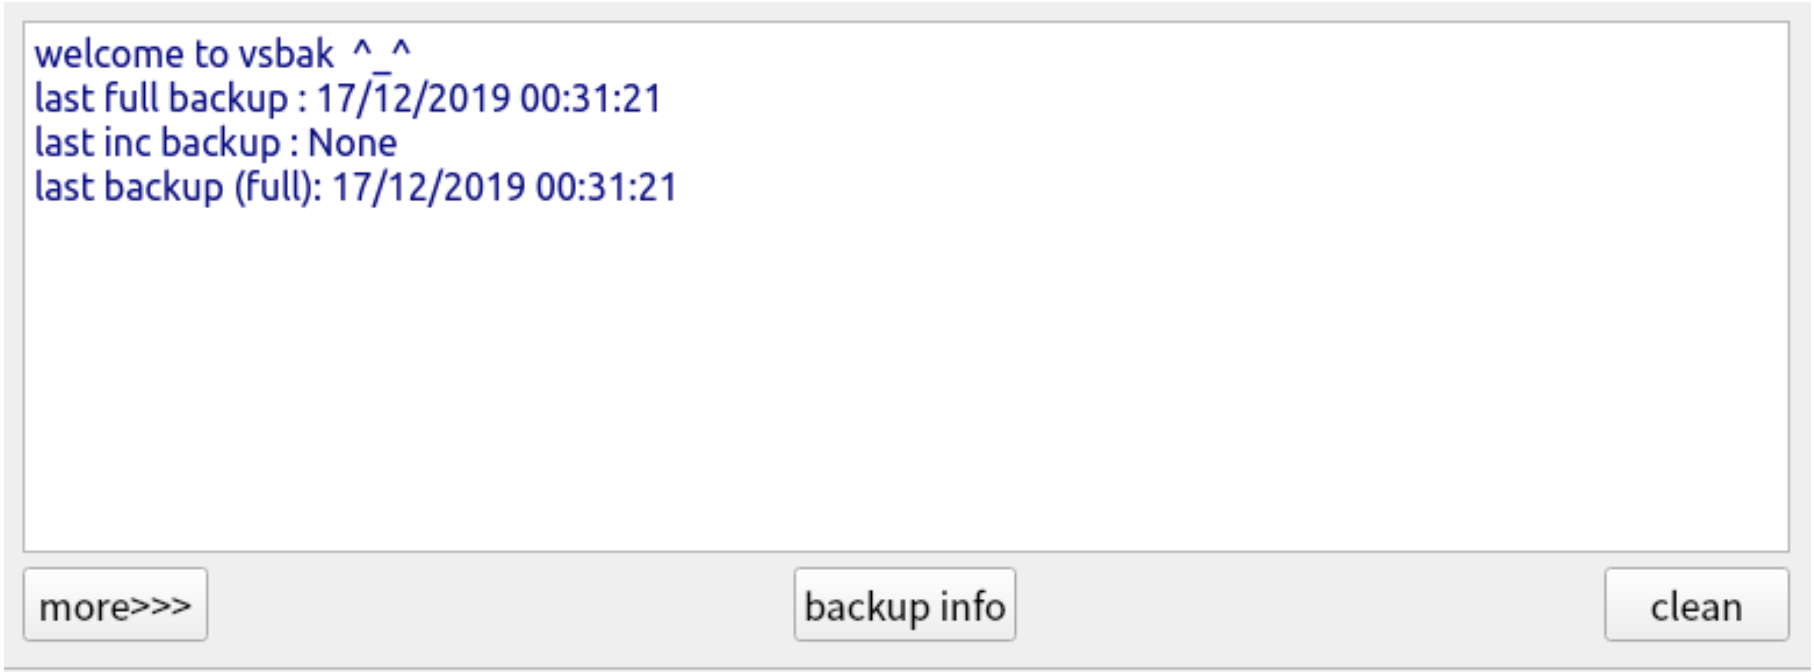
\includegraphics[width=0.8\textwidth]{bilder/backup_info.png}
	\caption{Der Bereich des Anzeigefeldes  }
	\label{Abbildung_7}
\end{figure}

Der Anzeigebereich zeigt das temporäre Protokoll nach jedem Schritt oder einen Hinweis auf dem nächsten Schritt. Das „clean“-Button räumt den Anzeigebereich. (s. Abbildung \ref{Abbildung_7}).

\begin{figure}[h!]
	\centering
	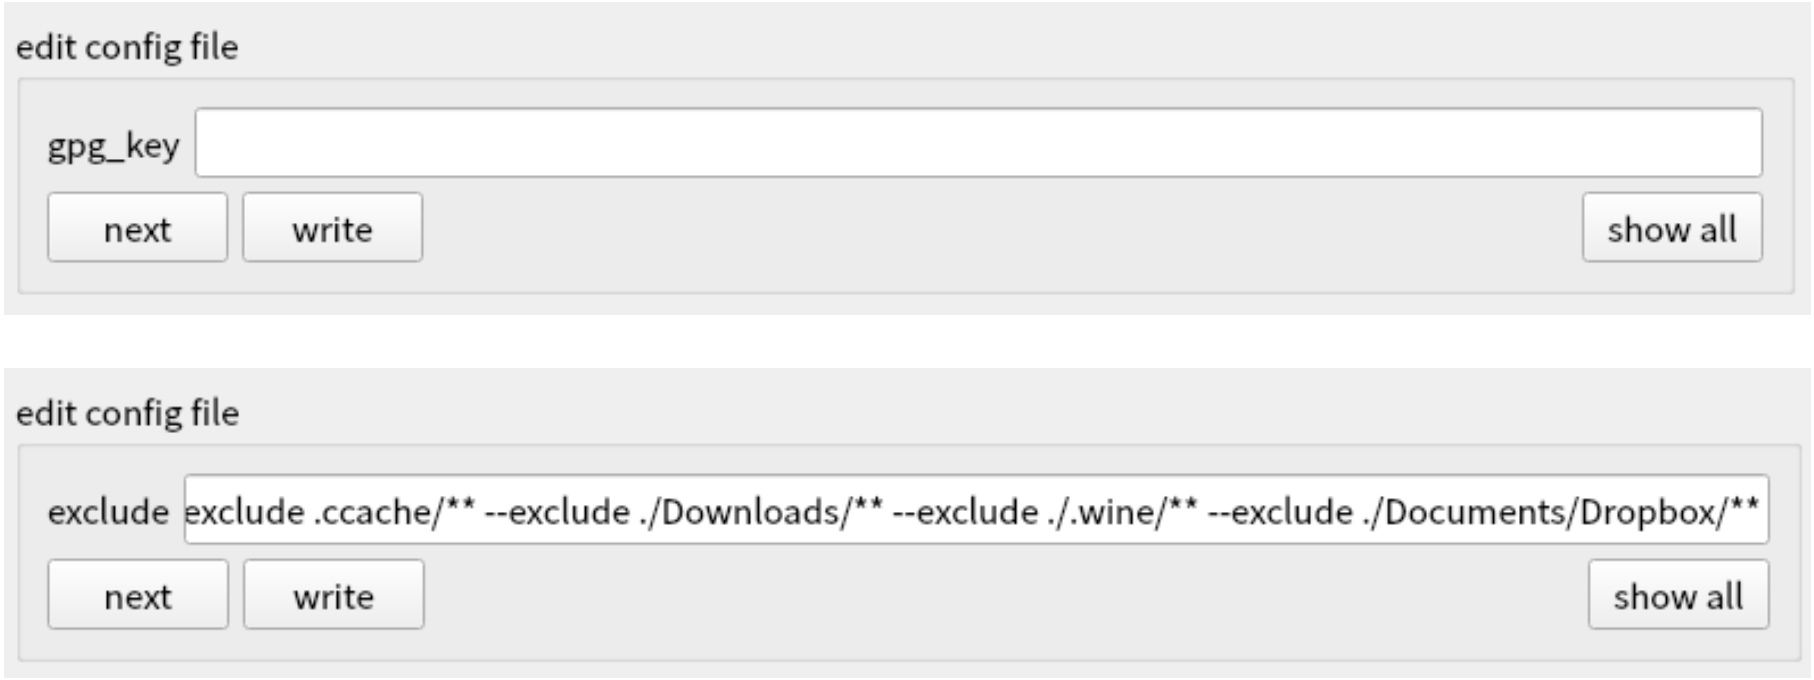
\includegraphics[width=0.8\textwidth]{bilder/more_func.png}
	\caption{Der Bereich der Erweiterung  }
	\label{Abbildung_8}
\end{figure}

Mit einem Klicken auf dem „more“-Button öffnet sich eine Erweiterung, in der man in einem Eingabefeld die „exclude“-Daten oder gpg-key der Konfigurationsdatei editieren kann. „Next“-Button sorgt für die Wechsel der zweien Edierungsmodi. Nach dem Klicken auf dem „write“-Button wird die Konfigurationsdatei nach der Eingabe von neuen „exclude“-Daten oder gewünschtem gpg-Key aktualisiert. „Show all“- Button schreibt den ganzen Inhalt der Konfigurationsdatei in das Anzeigefenster. (s. Abbildung \ref{Abbildung_8}). 

\section{Implementierung der Funktionen}

\begin{figure}[h!]
	\centering
	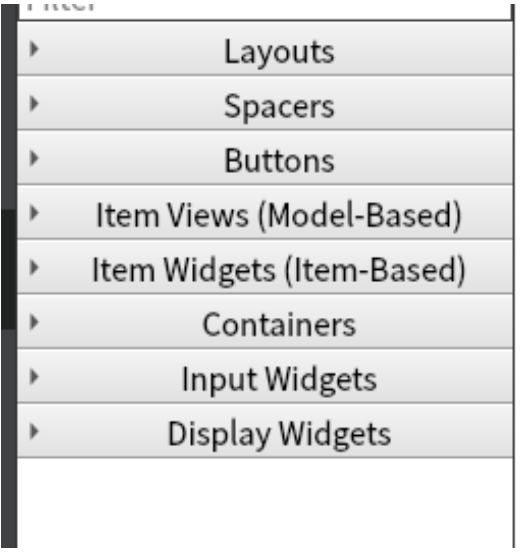
\includegraphics[width=0.3\textwidth]{bilder/widget.png}
	\caption{Das Verzeichnis der Widgets}
	\label{Abbildung_9}
\end{figure}

\begin{figure}[h!]
	\centering
	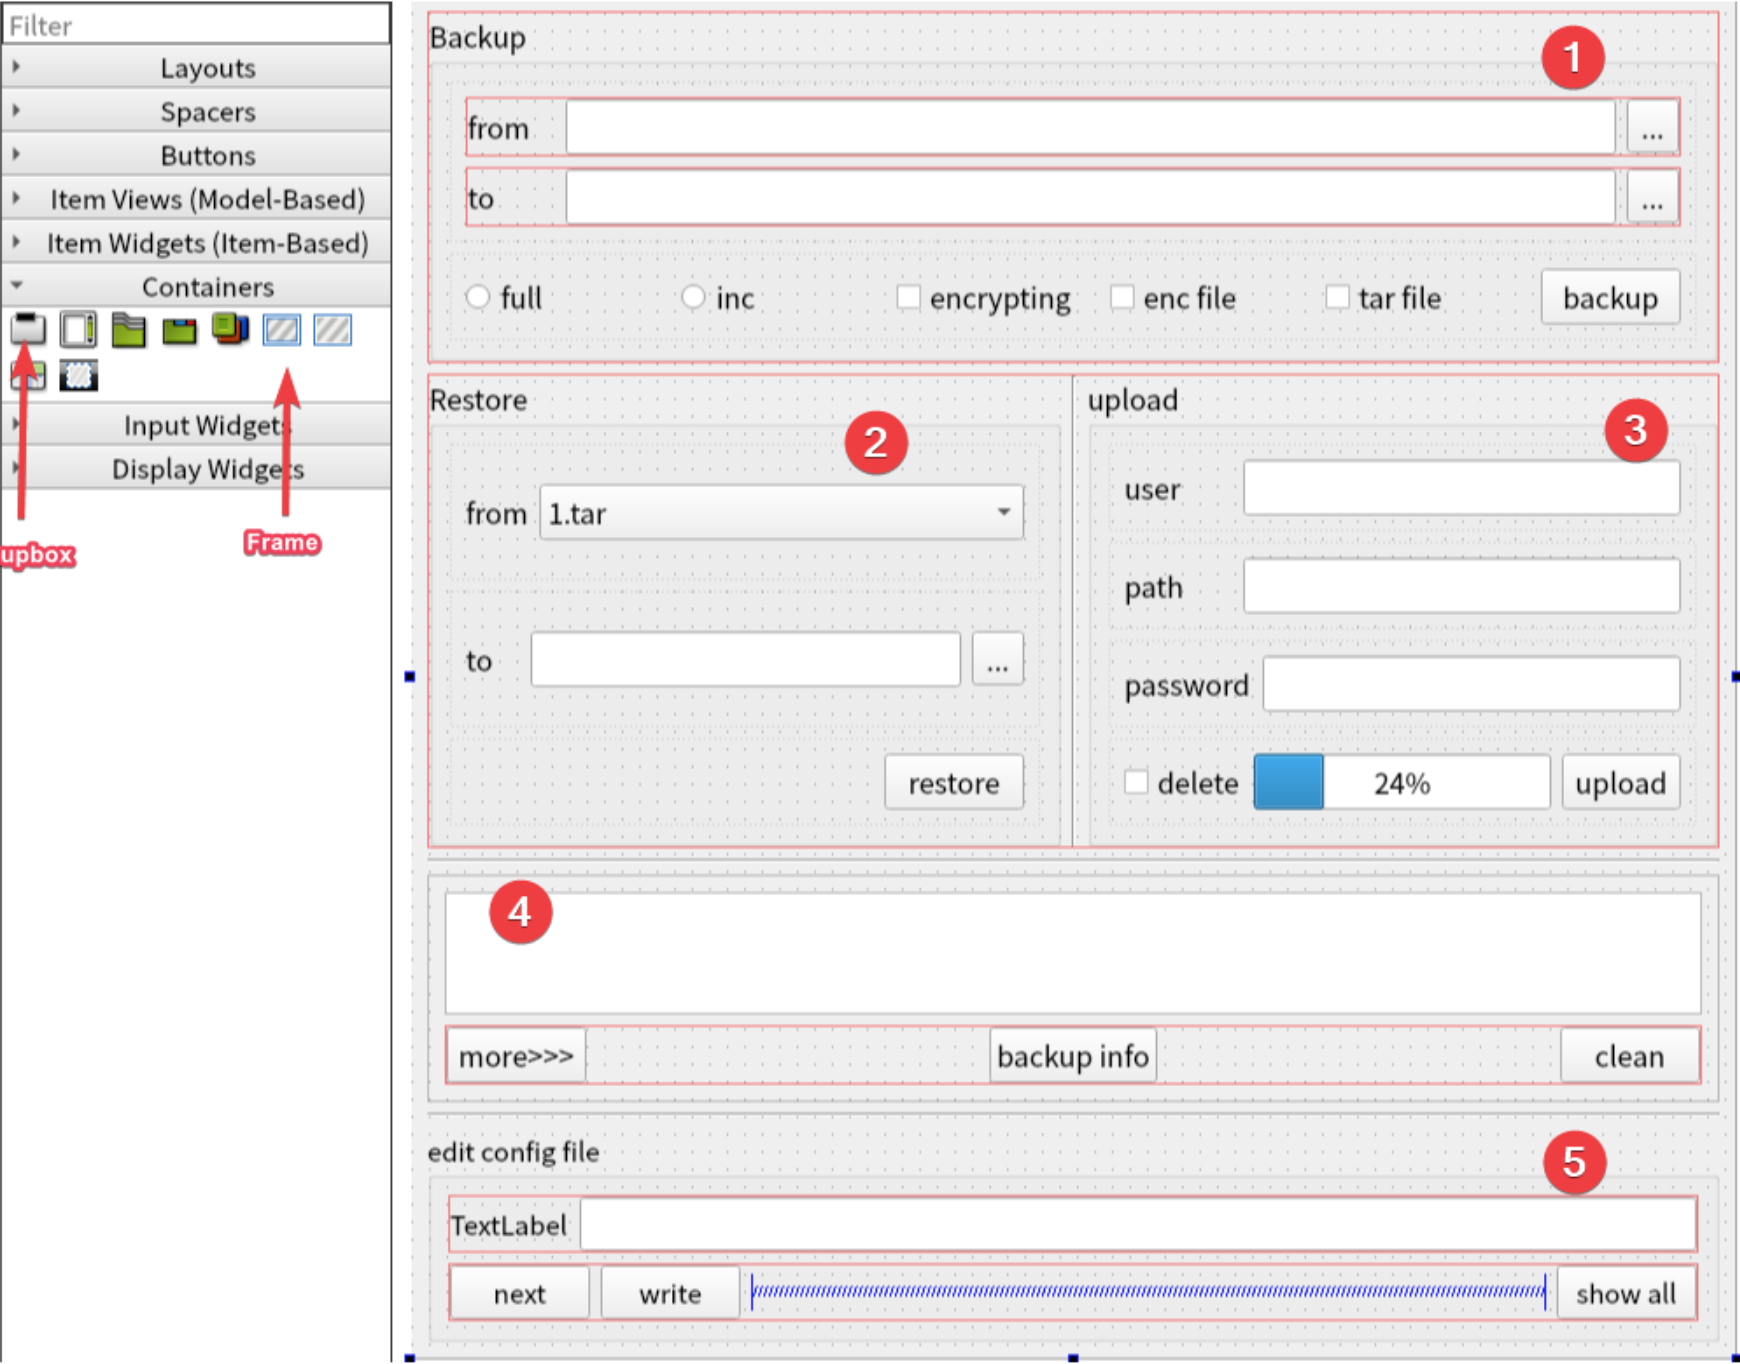
\includegraphics[width=0.9\textwidth]{bilder/edit_ui.png}
	\caption{Die Auslegung der grafischen Benutzeroberflaeche}
	\label{Abbildung_10}
\end{figure}

In UI-Designer werden Arbeitsoberflächen mit den zur Verfügung gestellten Widgets gestaltet, die nach Wunsch horizontal oder vertikal zusammengehört werden können. Am Beispiel werden die zweite und dritte Zone horizontal kombiniert. Im Wesentlich werden einzelne Widgets von einer Klasse Q-Widget abgeleitet. (s. Abbildung \ref{Abbildung_9} und \ref{Abbildung_10}).
Wie in Kapitel 3.1 beschrieben, gibt es fünf Zonen in der Arbeitsoberfläche. All die ausgewählten Widgets werden in vier Groupboxes und ein Frame (die fünfte Zone) eingelegt.

\begin{figure}[h!]
	\centering
	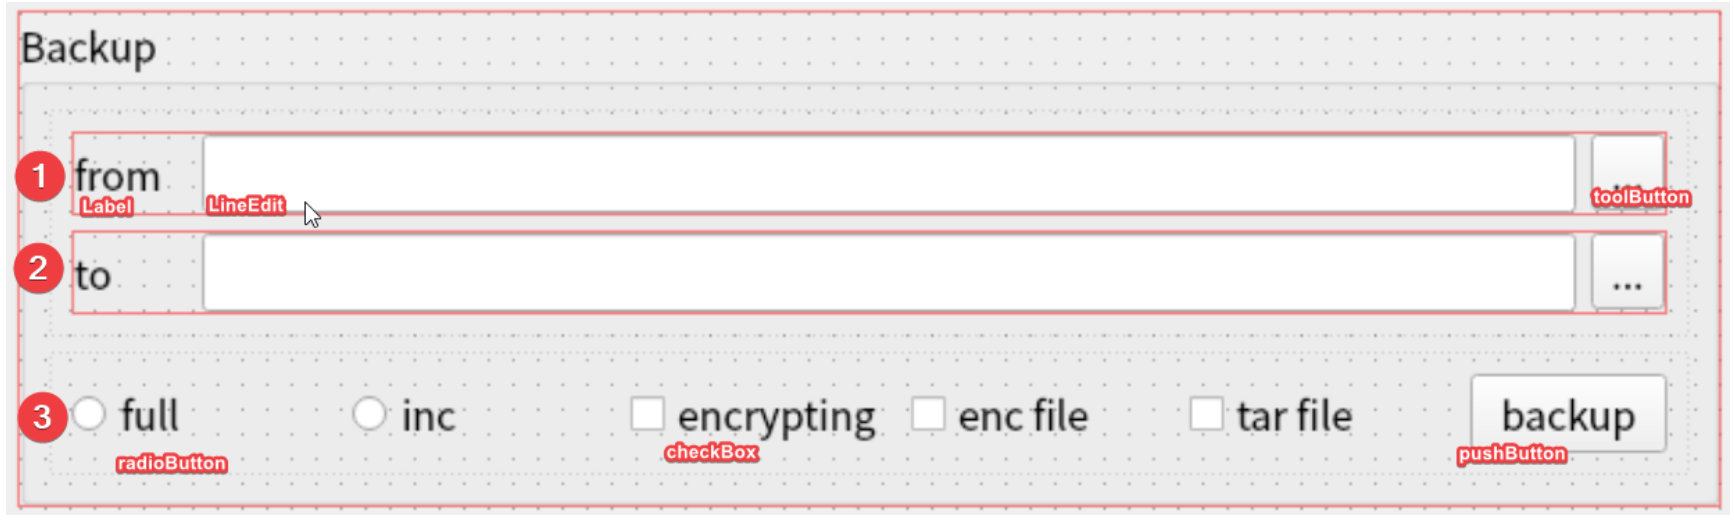
\includegraphics[width=0.9\textwidth]{bilder/man_backup.png}
	\caption{Die Auslegung des Bereichs des Backups }
	\label{Abbildung_11}
\end{figure}

Der erste Bereich besteht aus drei Zeilen, deren Widgets jeweils horizontal zusammengehören, und 6 Arten von Widgets, die folgendermaßen zur Beschreibung aufgelistet werden.  (s. Abbildung \ref{Abbildung_11}).
\begin{enumerate}
	\item Label: Im Label-Widget werden eine ersehnte Schrift als ein Label in einer bestimmten Stelle festgelegt. Am Beispiel in dem Programm weist das Label ``from'' darauf hin, wofür die Schriften, nämlich die Quelladresse, im LineEdit-Widget steht.  
	\item LineEdit: Im LineEdit-Widget wird die von dem ToolButton-Widget ausgewählte Quelladresse in dem Programm angezeigt.
	\item ToolButton: Ein ToolButton-Widget stellt ein Dialogfenster zur Auswahl der gewünschten Quelladresse im Laufe des Programms zur Verfügung. 
	\item RadioButton: Jedes RadioButton-Widget steht für eine funktionale Auswahl wie zum Beispiel das vollständige und inkrementelle Backup in dem Programm.
	\item CheckBox: Ein CheckBox-Widget, ist ausschließlich ein zusätzliche Auswahl aber nicht notwendig. In dem Programm werden ``enc file'' und ``tar file'' am Anfang automatisch angekreuzt, bevor die Auswahl ``encrypting'' angekreuzt wird. Nachdem die Auswahl ``encrpting'' angekreuzt wird, können ``enc file'' oder „tar file“ entfallen lassen. 
	\item PushButton: Mit einem Klick auf dem PushButton-Widget wird eine Funktion wie zum Beispiel Backup in diesem Projekt im Laufe des Programms nach den vorhergehenden Einstellungen dementsprechend aktiviert. 
\end{enumerate}

\begin{figure}[h!]
	\centering
	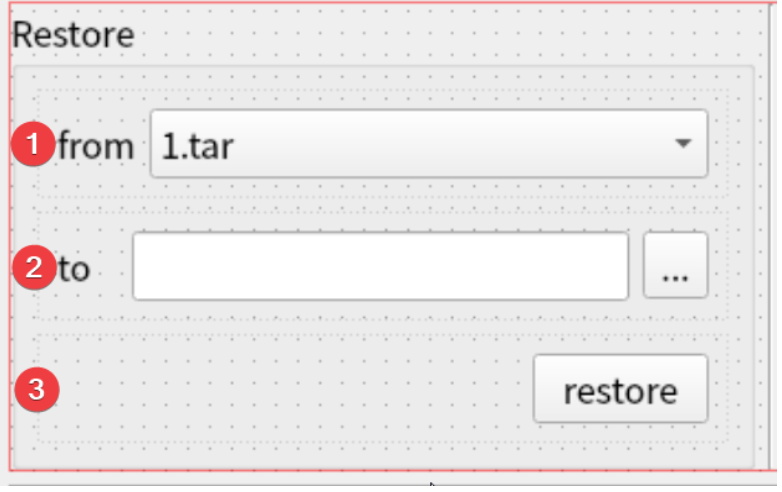
\includegraphics[width=0.4\textwidth]{bilder/man_restore.png}
	\caption{Die Auslegung des Bereichs des Restores }
	\label{Abbildung_12}
\end{figure}
Die Anordnung im Restore Bereich ist im ähnlich wie der erste Bereich. Anschließend kommt ein neues Widget, und zwar „ComBox“-Widget , vor, mit dem eine backupte Datei oder backuptes Dokument Zieladresse ausgewählt wird, um in irgendeinem Ort wiederherzustellen. (s.  Abbildung \ref{Abbildung_12}).

\begin{figure}[h!]
	\centering
	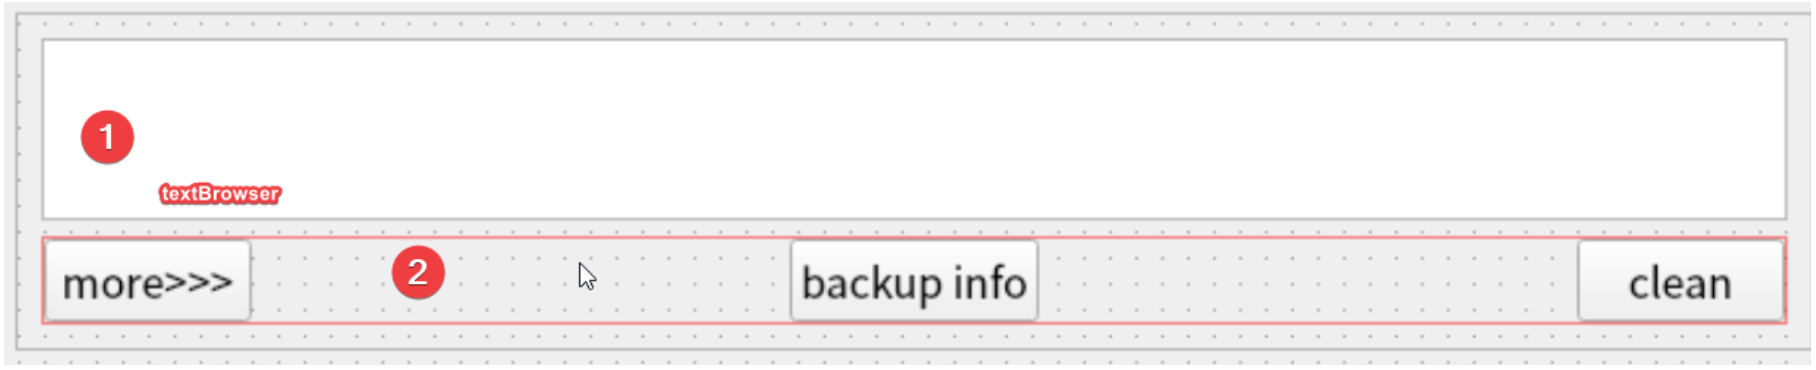
\includegraphics[width=0.8\textwidth]{bilder/man_info.png}
	\caption{Die Auslegung des Bereichs des Anzeigefeldes }
	\label{Abbildung_13}
\end{figure}
Im Bereich von Upload steht ein neues Widget, nämich „Progressbar“ als ein Fortschrittsbalken und die Anordnung ist gleich wie der zweite Bereich. Im vierten Bereich wird zwei Zeilen, deren Komponente jeweils ein „Textbrower“-Widget und drei „PushButton“-Widgets sind, gestaltet. Das „Textbrowser“-Widget spiegeln die detaillierten Hinweise auf die Bedienung in Schriften wider. (s. Abbildung \ref{Abbildung_13}).

\begin{figure}[h!]
	\centering
	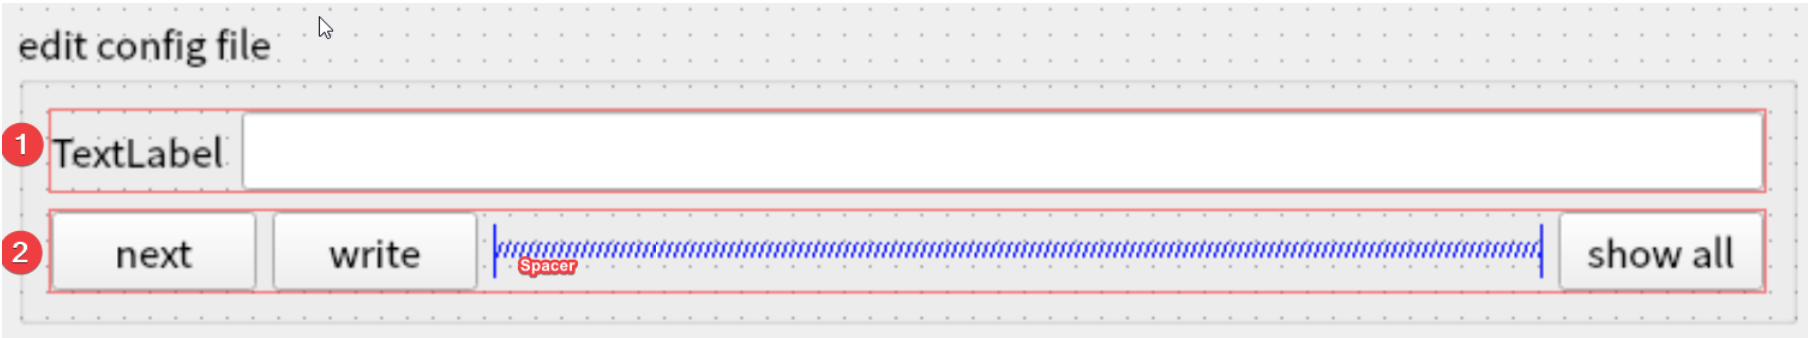
\includegraphics[width=0.8\textwidth]{bilder/man_more.png}
	\caption{Die Auslegung der Erweiterung }
	\label{Abbildung_14}
\end{figure}
In dem letzten Bereich wird nur ein neues Widget, also „Spacer“-Widget, zwishen zwei PushButtons gelegt, um einen richtigen Abstand zu halten.  (s. Abbildung \ref{Abbildung_14}).

\begin{figure}[h!]
	\centering
	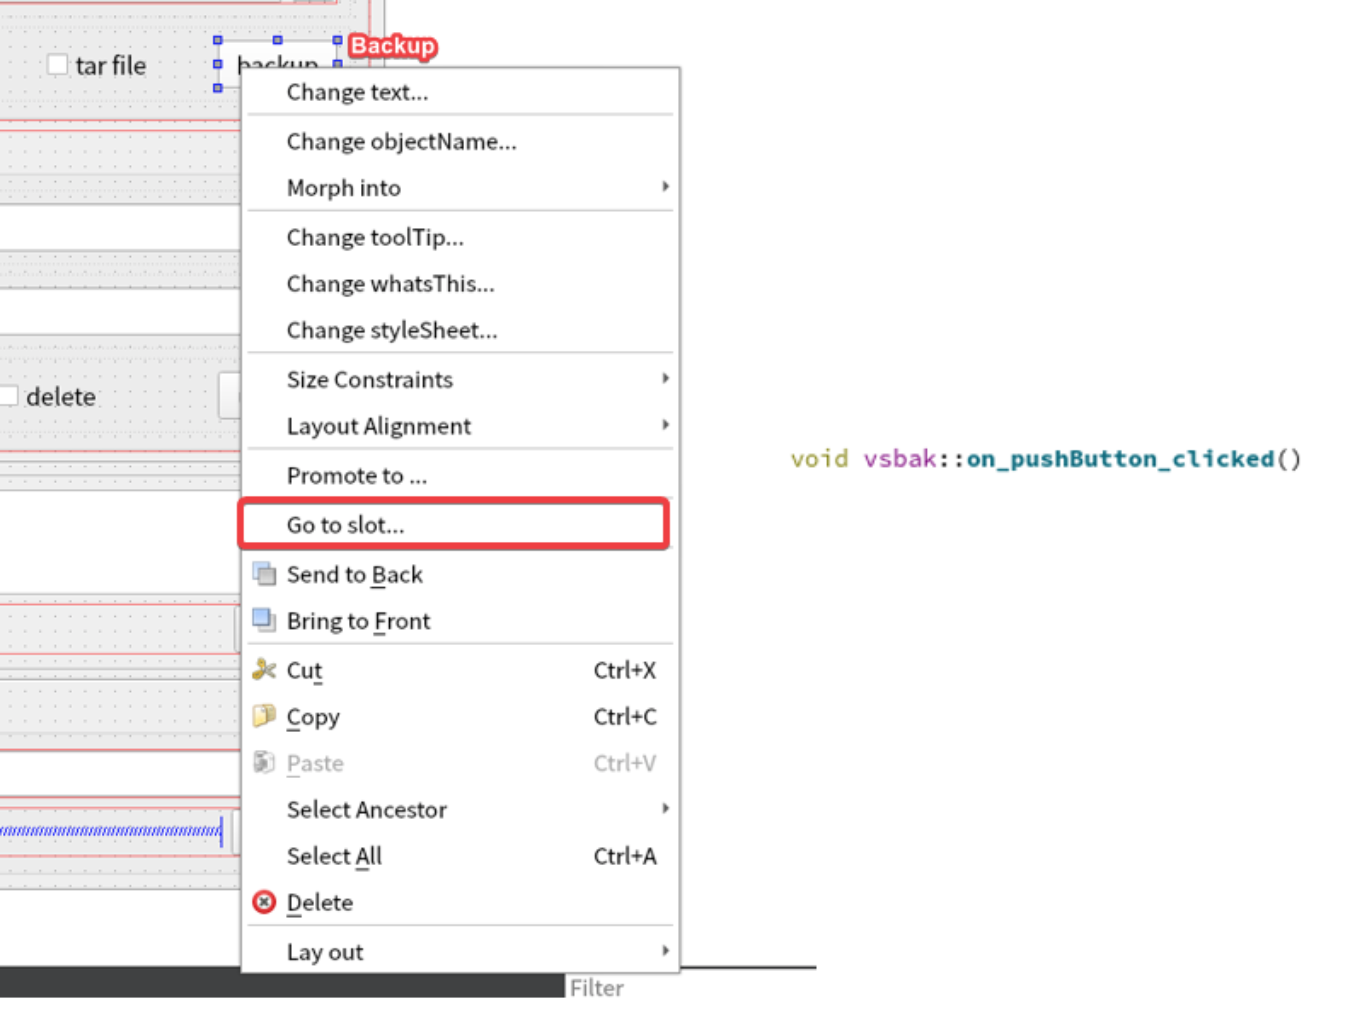
\includegraphics[width=0.4\textwidth]{bilder/slot.png}
	\caption{Die Funktionsdeklarationen von Slots }
	\label{Abbildung_15}
\end{figure}
Mit den angeordneten Layouts lassen sich die Funktionsdeklarationen von Slots in der Header-Datei und die Funktionsdefinitionen ohne Inhalte in der Cpp-Datei durch den Klick auf “go to slot” leicht sofort erstellt. (s. Abbildung \ref{Abbildung_15}). 


